\documentclass{standalone}

\usepackage{tikz}
\usetikzlibrary{calc}
\usetikzlibrary{decorations}
\usetikzlibrary{decorations.markings}

\begin{document}
  %noformat{
  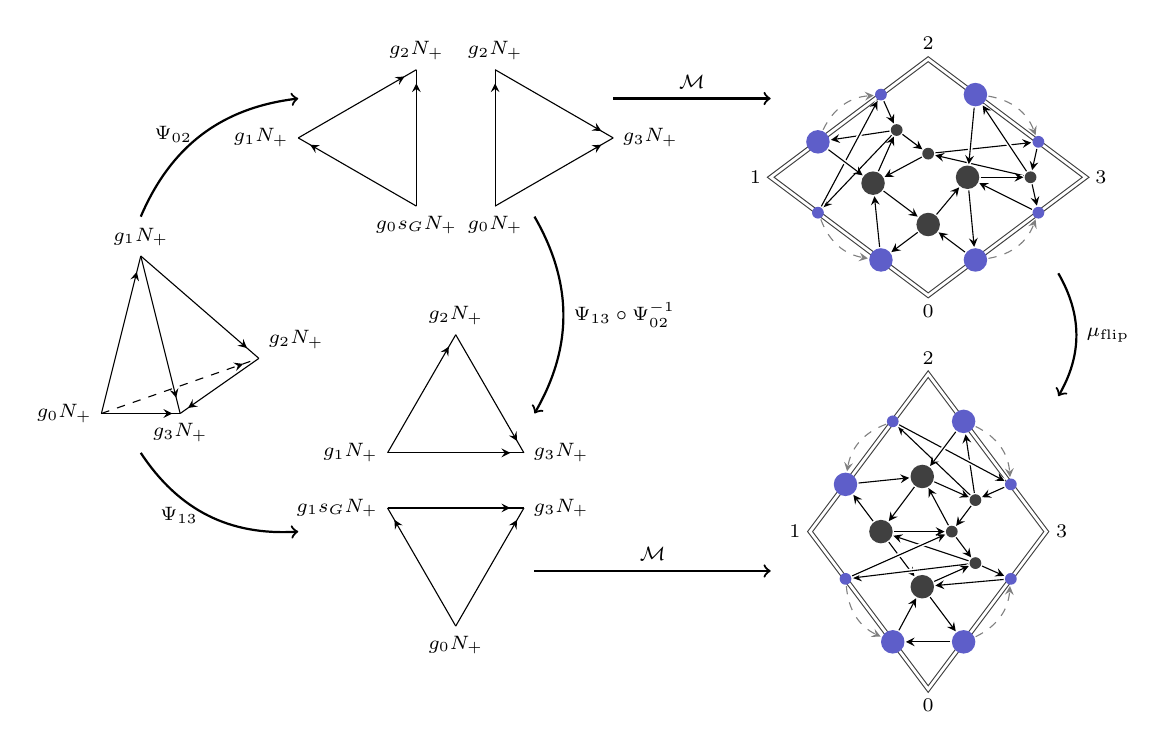
\begin{tikzpicture}
    \tikzstyle{v1} = [circle, outer sep=0.5pt, fill, inner sep=1.5pt]
    \tikzstyle{v2} = [circle, outer sep=0.5pt, fill, inner sep=3.0pt]
    \tikzstyle{unf} = [color=darkgray]
    \tikzstyle{frz} = [color=blue!60!darkgray!70]
    \tikzstyle{r} = [color=red!70!darkgray!70]
    \tikzstyle{e} = [->, >={stealth}, preaction={draw=white, -, ultra thick}]
    \tikzstyle{b} = [fill, fill opacity=0.0, circle, outer sep=0.5pt, inner sep=1.5pt]
    \tikzstyle{te} = [color=darkgray, double distance=1pt]
    \tikzstyle{h} = [dashed, color=gray, ->, >={stealth}]
    \tikzstyle{se} = [postaction=decorate, decoration={markings, mark=at position 0.9 with {\arrow{stealth}}}]

    \tikzset{font=\scriptsize}

    \begin{scope}[shift={(-1.5,1.0)}]
      \coordinate[label=180:{$g_0N_{+}$}] (v0) at (0.0,0.0);
      \coordinate[label= 90:{$g_1N_{+}$}] (v1) at (0.5,2.0);
      \coordinate[label= 30:{$g_2N_{+}$}] (v2) at (2.0,0.7);
      \coordinate[label=270:{$g_3N_{+}$}] (v3) at (1.0,0.0);

      \draw[se] (v0) to (v1);
      \draw[dashed, se] (v0) to (v2);
      \draw[se] (v0) to (v3);
      \draw[se] (v1) to (v2);
      \draw[se] (v1) to (v3);
      \draw[se] (v2) to (v3);
    \end{scope}

    \begin{scope}[shift={(3.0,4.5)}]
      \coordinate[label=270:{$g_0 s_G N_{+}$}] (vl0) at ($ (300:1.0) + (180:1.0) $);
      \coordinate[label=180:{$g_1 N_{+}$}]     (vl1) at ($ (180:1.0) + (180:1.0) $);
      \coordinate[label= 90:{$g_2 N_{+}$}]     (vl2) at ($ ( 60:1.0) + (180:1.0) $);
      \draw[se] (vl0) to (vl1);
      \draw[se] (vl1) to (vl2);
      \draw[se] (vl0) to (vl2);

      \coordinate[label=270:{$g_0N_{+}$}]     (vr0) at ($ (240:1.0) + (  0:1.0) $);
      \coordinate[label=  0:{$g_3N_{+}$}]     (vr2) at ($ (  0:1.0) + (  0:1.0) $);
      \coordinate[label= 90:{$g_2N_{+}$}]     (vr1) at ($ (120:1.0) + (  0:1.0) $);
      \draw[se] (vr0) to (vr1);
      \draw[se] (vr1) to (vr2);
      \draw[se] (vr0) to (vr2);
    \end{scope}

    \begin{scope}[shift={(3.0,0.0)}]
      \coordinate[label=180:{$g_1N_{+}$}]     (vl0) at ($ (210:1.0) + ( 90:1.0) $);
      \coordinate[label= 90:{$g_2N_{+}$}]     (vl1) at ($ ( 90:1.0) + ( 90:1.0) $);
      \coordinate[label=  0:{$g_3N_{+}$}]     (vl2) at ($ (330:1.0) + ( 90:1.0) $);
      \draw[se] (vl0) to (vl1);
      \draw[se] (vl1) to (vl2);
      \draw[se] (vl0) to (vl2);

      \coordinate[label=270:{$g_0N_{+}$}]     (vr0) at ($ (270:1.0) + (270:0.7) $);
      \coordinate[label=180:{$g_1 s_GN_{+}$}] (vr1) at ($ (150:1.0) + (270:0.7) $);
      \coordinate[label=  0:{$g_3N_{+}$}]     (vr2) at ($ ( 30:1.0) + (270:0.7) $);
      \draw[se] (vr0) to (vr1);
      \draw[se] (vr1) to (vr2);
      \draw[se] (vr0) to (vr2);
    \end{scope}

    \begin{scope}[shift={(9,4)}]
      % Copied from fig-dv-construction.tex
      \coordinate[label=270:{$0$}] (q_0) at (270:1.5);
      \coordinate[label=180:{$1$}] (q_1) at (180:2.0);
      \coordinate[label= 90:{$2$}] (q_2) at ( 90:1.5);
      \coordinate[label=  0:{$3$}] (q_3) at (  0:2.0);

      \draw[te] (q_0) -- (q_1) -- (q_2) -- (q_3) -- cycle;
 
      \node[v2, frz] (D1) at    ($ (q_0)!0.30!(q_1) $) {};
      \node[v1, frz] (D2) at    ($ (q_0)!0.70!(q_1) $) {};

      \node[v2, frz] (E1) at    ($ (q_1)!0.30!(q_2) $) {};
      \node[v1, frz] (E2) at    ($ (q_1)!0.70!(q_2) $) {};

      \node[v2, frz] (F1) at    ($ (q_2)!0.30!(q_3) $) {};
      \node[v1, frz] (F2) at    ($ (q_2)!0.70!(q_3) $) {};

      \node[v2, frz] (G1) at    ($ (q_0)!0.30!(q_3) $) {};
      \node[v1, frz] (G2) at    ($ (q_0)!0.70!(q_3) $) {};

      \coordinate (e01mid) at ($ (q_0)!0.5!(q_1) $);

      \node[v2, unf] (w11) at ($ (q_3) + (180:1.5)$) {};
      \node[v1, unf] (w21) at ($ (q_3) + (180:0.7)$) {};

      \node[v2, unf] (w12) at ($ (q_2)!0.7!(q_0) $) {};
      \node[v1, unf] (w22) at ($ (q_2)!0.4!(q_0) $) {};

      \node[v2, unf] (w13) at ($ (q_2)!0.7!(e01mid) $) {};
      \node[v1, unf] (w23) at ($ (q_2)!0.4!(e01mid) $) {};

      \draw[h]  (D2) to[bend right] (D1);
      \draw[h]  (E1) to[bend left]  (E2);
      \draw[h]  (F1) to[bend left]  (F2);
      \draw[h]  (G1) to[bend right] (G2);

      \draw[e] (D1) -- (w13);
      \draw[e] (w23) -- (w22);
      \draw[e] (w23) -- (D2);
      \draw[e] (w23) -- (E1);
      \draw[e] (w12) -- (D1);
      \draw[e] (w12) -- (w11);
      \draw[e] (w22) -- (w13);
      \draw[e] (w22) -- (F2);
      \draw[e] (E2) -- (w23);
      \draw[e] (D2) -- (E2);
      \draw[e] (w13) -- (w23);
      \draw[e] (w13) -- (w12);
      \draw[e] (E1) -- (w13);
      \draw[e] (w21) -- (w22);
      \draw[e] (w21) -- (G2);
      \draw[e] (w21) -- (F1);
      \draw[e] (G1) -- (w12);
      \draw[e] (G2) -- (w11);
      \draw[e] (F2) -- (w21);
      \draw[e] (w11) -- (w21);
      \draw[e] (w11) -- (G1);
      \draw[e] (F1) -- (w11);
    \end{scope}


    \begin{scope}[shift={(9,-0.50)}]
      \coordinate[label=270:{$0$}] (q_0) at (270:2.0);
      \coordinate[label=180:{$1$}] (q_1) at (180:1.5);
      \coordinate[label= 90:{$2$}] (q_2) at ( 90:2.0);
      \coordinate[label=  0:{$3$}] (q_3) at (  0:1.5);

      \draw[te] (q_0) -- (q_1) -- (q_2) -- (q_3) -- cycle;
 
      \node[v2, frz] (D1) at    ($ (q_0)!0.30!(q_1) $) {};
      \node[v1, frz] (D2) at    ($ (q_0)!0.70!(q_1) $) {};

      \node[v2, frz] (E1) at    ($ (q_1)!0.30!(q_2) $) {};
      \node[v1, frz] (E2) at    ($ (q_1)!0.70!(q_2) $) {};

      \node[v2, frz] (F1) at    ($ (q_2)!0.30!(q_3) $) {};
      \node[v1, frz] (F2) at    ($ (q_2)!0.70!(q_3) $) {};

      \node[v2, frz] (G1) at    ($ (q_0)!0.30!(q_3) $) {};
      \node[v1, frz] (G2) at    ($ (q_0)!0.70!(q_3) $) {};

      \coordinate (e12mid) at ($ (q_1)!0.5!(q_2) $);
      \coordinate (e01mid) at ($ (q_0)!0.5!(q_1) $);

      \node[v2, unf] (w11) at ($ (q_3)!0.7!(e12mid) $) {};
      \node[v1, unf] (w21) at ($ (q_3)!0.4!(e12mid) $) {};

      \node[v2, unf] (w12) at ($ (q_3)!0.7!(q_1) $) {};
      \node[v1, unf] (w22) at ($ (q_3)!0.4!(q_1) $) {};

      \node[v2, unf] (w13) at ($ (q_3)!0.7!(e01mid) $) {};
      \node[v1, unf] (w23) at ($ (q_3)!0.4!(e01mid) $) {};

      \draw[h]  (D2) to[bend right] (D1);
      \draw[h]  (E2) to[bend right] (E1);
      \draw[h]  (F1) to[bend left]  (F2);
      \draw[h]  (G1) to[bend right] (G2);

      \draw[e] (E1) -- (w11);
      \draw[e] (w21) -- (w22);
      \draw[e] (w21) -- (E2);
      \draw[e] (w21) -- (F1);
      \draw[e] (w12) -- (E1);
      \draw[e] (w12) -- (w22);
      \draw[e] (w12) -- (w13);
      \draw[e] (w22) -- (w11);
      \draw[e] (w22) -- (w23);
      \draw[e] (F2) -- (w21);
      \draw[e] (E2) -- (F2);
      \draw[e] (w11) -- (w21);
      \draw[e] (w11) -- (w12);
      \draw[e] (F1) -- (w11);
      \draw[e] (D1) -- (w13);
      \draw[e] (w23) -- (w12);
      \draw[e] (w23) -- (G2);
      \draw[e] (w23) -- (D2);
      \draw[e] (G1) -- (D1);
      \draw[e] (G2) -- (w13);
      \draw[e] (D2) -- (w22);
      \draw[e] (w13) -- (w23);
      \draw[e] (w13) -- (G1);
    \end{scope}

    \draw[->, thick] (-1.0, 3.5) to[bend left ] node[midway, left] (t01) {$\Psi_{02}$} ( 1.0, 5.0);
    \draw[->, thick] (-1.0, 0.5) to[bend right] node[midway, left] (t02) {$\Psi_{13}$} ( 1.0,-0.5);
    \draw[->, thick] ( 4.0,-1.0) to node[midway, above] (t03) {$\mathcal{M}$} ( 7.0,-1.0);
    \draw[->, thick] ( 5.0, 5.0) to node[midway, above] (t04) {$\mathcal{M}$} ( 7.0, 5.0);
    \draw[->, thick] ( 4.0, 3.5) to[bend left ] node[midway, right] (t05) {$\Psi_{13} \circ \Psi_{02}^{-1}$} ( 4.0, 1.0);
    \draw[->, thick]
        ($ (9,4) + (  0:2.598)!0.5!(270:1.7321) + (315:0.5) $)
        to[bend left] node[midway, right] (t06) {$\mu_{\mathrm{flip}}$}
        ($ (9,0) + (  0:2.598)!0.5!( 90:1.7321) + ( 45:0.5) $);
  \end{tikzpicture}
  %}noformat
\end{document}
